\subsection{Wavelet Analysis}
Wavelet analysis is a generalization of Fourier analysis which breaks the signal into series of sines and cosines. This transformation reveals the frequency space properties but loses all the temporal information. \cite{Fong04} A Fourier transform of a function $x(t)$ is 
\begin{equation}
F_{x}(t) = a_0 + \sum_{k=1}^{\infty} a_k cos(kt) + b_k sin(kt),
\end{equation}

where
\begin{align}
a_0 &= \frac{1}{2\pi} \int_{0}^{2\pi} x(t) dt \\
a_k &= \frac{1}{\pi} \int_{0}^{2\pi} x(t) cos(kt) dt \\
b_k &= \frac{1}{\pi} \int_{0}^{2\pi} x(t) sin(kt) dt.
\end{align}

This corresponds to a mapping into the frequency space that is formed by orthogonal basis functions, sine and cosine. By orthogonality we mean that for a set of signals $\psi_n(t)$, $-\infty < n < \infty$, we have
\begin{equation}
\left \langle \psi_n(t), \psi_m(t) \right \rangle = 0, \; m \ne n
\end{equation}

We can generalize the idea of Fourier transform into any orthogonal basis of signals $\psi_n(t)$. The analysis part calculates the coefficients of the original signal $x(t)$ in the new space:
\begin{equation}
c_n = \frac{\left \langle x(t), \psi_n(t) \right \rangle}{\left \langle \psi_n(t), \psi_n(t) \right \rangle}.
\end{equation}

Then, the original signal can be constructed from the coefficients by
\begin{equation}
x(t) = \sum_{n=-\infty}^{\infty} c_n \psi_n(t),
\end{equation}
which is called the synthesis process.

Fourier transform reveals the frequency band of the signal while losing all the temporal information about different frequencies. \cite{Fong04} Because of this Fourier transform is applicable only to stationary signals $f(t)$ whose variance does not vary with time. No information about the changes in variance are captured by Fourier transformation and hence the method becomes useless with non-stationary signals. Anomalies in time series data cause spectral variance and hence the signal is not stationary. \cite{Hautakangas11} 

We can define the short time Fourier transform (STFT) as
\begin{equation}
\operatorname{STFT}(f, s) = \int_{-\infty}^{\infty} x(t) g(t-s) e^{-j 2\pi ft} dt,
\end{equation}
where $f$ is frequency of $x(t)$ and $g(t)$ is a sliding window function, for example, a box function
\begin{equation}
\operatorname{box}(t) = 
\begin{cases}
1 & \text{for} \; |t| \le 1/2 \\
0 & \text{elsewhere}
\end{cases}.
\end{equation}

This restricts the Fourier transform into one window at the time and thus achieves time-localization which the ordinary Fourier transform lacks of. For computational purposes we must discretize this by denoting $f_n = n/T$ and $s_m = mT$. In this case our orthogonal basis functions are
\begin{equation}
v_{n,m} (t) = e^{j 2\pi nt / T} g(t - mT).
\end{equation}

Now the analysis part is
\begin{align}
c_{n,m} &= \frac{\left \langle x(t), v_{n,m}(t) \right \rangle}{\left \langle v_{n,m}(t), v_{n,m}(t) \right \rangle} \\
&= \frac{1}{T} \int_{mT}^{(m+1)T} x(t) e^{-j 2\pi nt / T} dt
\end{align}
and the synthesis is 
\begin{equation}
x(t) = \sum_{n=-\infty}^{\infty} \sum_{m=-\infty}^{\infty} c_{n,m} e^{j 2\pi nt / T} g(t - mT).
\end{equation}

Unlike Fourier transform, wavelet transformation gives the signal localization in both time and frequency spaces. It does this by using a concept called multi-resolution analysis (MRA) which means that different frequencies are analyzed with different resolutions. While Fourier transformation uses equally-sized windows for all frequencies, Wavelet transformation uses longer time windows for low frequencies and shorter time windows for high frequencies. This approach allows good localization of high frequency components while preserving information about low frequency contents of the signal. \cite{Fong04}

Continuous wavelet transform (CWT) for signal $x(t)$ is defined as
\begin{equation}
C_{x}(a,b) = \frac{1}{\sqrt{|a|}} \int_{-\infty}^{\infty} x(t) w \left ( \frac{t - b}{a} \right ) dt,
\end{equation}
where $a$ and $b$ are scaling and positioning parameters and $w(t)$ is a so-called mother wavelet function. \cite{Fong04} 

For computational purposes we must find a discrete wavelet transform (DWT). By choosing the scales to be powers of 2 and the positions to be multiples of the scales, we get an orthogonal basis of functions for CWT:
\begin{equation}
w_{j,k}(t) = 2^{j/2} w(2^j t - k).
\end{equation}

These $w_{j,k}(t)$ are called the baby wavelets. \cite{Phillips03} As can be easily seen, baby wavelets become narrower and higher as the $j$ increases. The reverse is also true, baby wavelets become wider and flatter as the $j$ decreases. We can now define space $W_j$ to contain all the signals $x_j(t)$ that can be synthesized from baby wavelets $w_{j,k}(t)$ with the $j$ fixed:
\begin{equation}
x_j(t) = \sum_{k=-\infty}^{\infty} c_{j,k} w_{j,k}(t).
\end{equation}

Similarly, let $V_j$ to be the space of signals $x(t)$ that can be synthesized from baby wavelets $w_{i,k}(t)$ where $i < j$ and $-\infty < k < \infty$. Then, from the definition of $W_j$ and $V_j$ we have $V_{j+1} = W_j + V_j$. This is illustrated in figure~\ref{fig:wavelet_spaces}.


\begin{figure}[here]
\centering
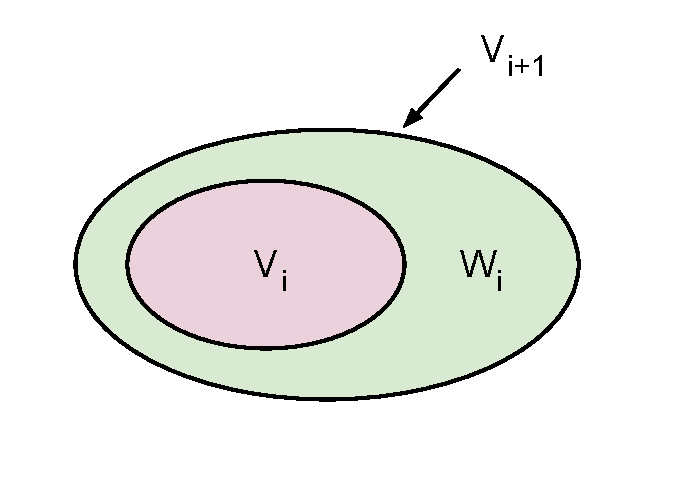
\includegraphics[scale=0.7]{images/wavelet_spaces.pdf}
\caption{Wavelet subspaces.}
\label{fig:wavelet_spaces}
\end{figure}

Thus, the spaces $V_j$ are nested inside each other, that is $\{0\} \subset \ldots \subset V_{-1} \subset V_{0} \subset V_{1} \subset \ldots L^2$, where $L^2$ contains all possible signals. The spaces $W_j$ are the differences between adjacent spaces $V_j$ and $V_{j+1}$. Now we can divide the space $V_0$ as
\begin{align*}
V_0 &= V_{-1} + W_{-1} \\
&= V_{-2} + W_{-2} + W_{-1} \\
&= V_{-3} + W_{-3} + W_{-2} + W_{-1} \\
&= \cdots
\end{align*}
and the signal as
\begin{align}
x(t) &= A_1(t) + D_1(t) \label{eq:decomposition} \\
&= A_2(t) + D_2(t) + D_1(t) \\
&= A_3(t) + D_3(t) + D_2(t) + D_1(t) \\
&= \cdots,
\end{align}
where $D_i(t) \in W_{-i}$ is the detail at level $i$ and $A_i(t) \in V_{-i}$ is the approximation at level $i$. This approach is called multi-resolution analysis (MRA) because on each step we divide the frequency band into two pieces and then continue the process on the lower half. At each stage the $A_i(t)$ corresponds to low-pass filtered signal and the $D_i(t)$ to high-pass filtered signal. This way we get more detailed information about the high frequencies. \cite{Phillips03} 

To facilitate the computations we can define a scaling function $\phi(t)$ (sometimes called the father wavelet) which produces the subspaces $V_j$:
\begin{equation}
\phi_{j,k}(t) = \sqrt{2^j} \phi(2^j t - k).
\end{equation}

Because $V_0 \subset V_1$ and $W_0 \subset V_1$, it is possible to construct the mother wavelet and the scaling function in $V_1$ from the scaling function in $V_0$ as follows
\begin{align}
\phi(t) &= \sum_n h_0(n) \sqrt{2} \phi(2t - n) \\
w(t) &= \sum_n h_1(n) \sqrt{2} \phi(2t - n),
\end{align}
where $h_0(n)$ and $h_1(n)$ are discrete time filter coefficients. These depend on the choice of wavelet type and they will be defined later. Now we are able to define the signal $x(t) \in V_j$ using the mother wavelet and the scaling function in spaces $V_{j-1}$ and $W_{j-1}$
\begin{align}
x(t) &= \sum_k cA_0(k) \phi_{j,k}(t) \\
&= \sum_k cA_1(k) \phi_{j-1,k}(t) + \sum_k cD_1(k) w_{j-1,k}(t) \\
&= A_1(t) + D_1(t),
\end{align}
where $cA_0(k)$, $cA_1(k)$ and $cD_1(k)$ are the approximate and detail coefficients respectively. Then, $\phi_{j-1,k}$ can be further filtered to get the next level signals as shown in equation~\ref{eq:decomposition}. The coefficient values can be derived as follows
\begin{align}
cA_1(k) &= \left \langle x(t), \phi_{j-1,k}(t) \right \rangle \\
		&= \left \langle \sum_n cA_0(n) \phi_{j,n}(t), \phi_{j-1,k}(t) \right \rangle \\
		&= \sum_n cA_0(n) \left \langle \phi_{j,n}(t), \phi_{j-1,k}(t) \right \rangle,
\end{align}
which, by calculating the inner product simplifies to
\begin{align}
cA_1(k) = \sum_n h_0(n-2k) cA_0(n)
\end{align}

Similarly, for $cD_1(k)$ we get
\begin{align}
cD_1(k) = \sum_n h_1(n-2k) cA_0(n)
\end{align}

These two operations correspond to filters
\begin{align}
&cA_0(n) \longrightarrow \boxed{h_0(-n)} \longrightarrow \boxed{\downarrow 2} \longrightarrow cA_1(k) \label{eq:downsampling1} \\
&cA_0(n) \longrightarrow \boxed{h_1(-n)} \longrightarrow \boxed{\downarrow 2} \longrightarrow cD_1(k), \label{eq:downsampling2}
\end{align}
where the downsampling filter, $\boxed{\downarrow 2}$, means omitting every other value from the signal. As shown in equation~\ref{eq:decomposition}, we can further use the downsampling filters to decompose the signal into more detail. This process is shown in Figure~\ref{fig:wavelet_filters}.

\begin{figure}[here]
\centering
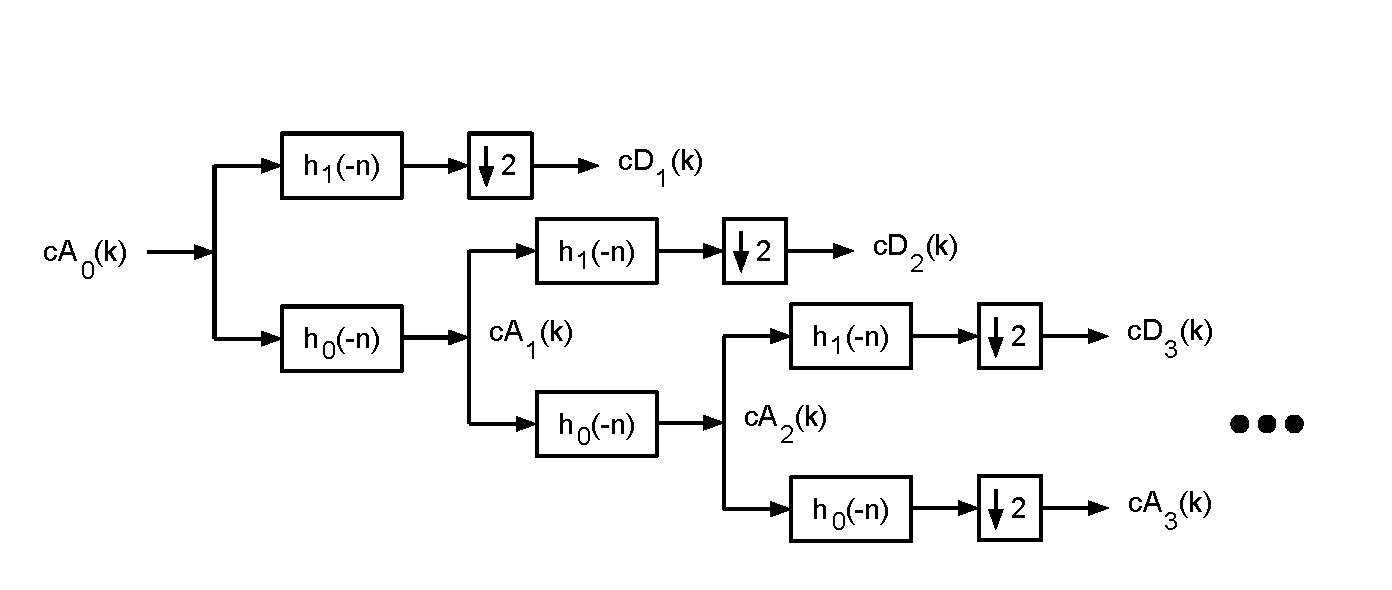
\includegraphics[scale=0.7]{images/wavelet_filters.pdf}
\caption{Wavelet coefficient decomposition using filters.}
\label{fig:wavelet_filters}
\end{figure}

Now on level $N$ our coefficients are
\begin{align}
C = [cA_N, cD_N, cD_{N-1}, ..., cD_2, cD_1]
\end{align}

The signal is now compressed by setting some of the detail coefficients to zero. Of course, the energy of the signal is not completely preserved and the number of zero coefficients depends on the application.

Next, we need to perform the synthesis part by opposite, upsampling filters. This process is shown in Figure~\ref{fig:wavelet_filters2}.

\begin{figure}[here]
\centering
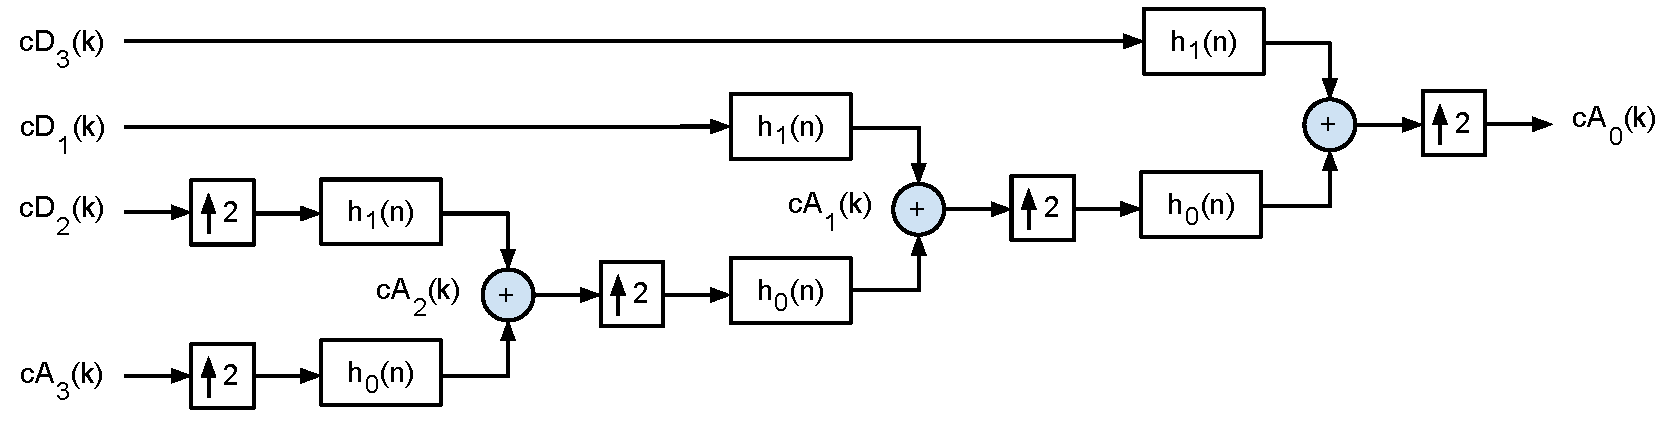
\includegraphics[scale=0.55]{images/wavelet_filters2.pdf}
\caption{Wavelet coefficient decomposition using filters.}
\label{fig:wavelet_filters2}
\end{figure}

If no coefficients are set to zero in the analysis phase, the signal that is constructed in the synthesis phase is exactly the same as the original signal. By setting some of the detail coefficients to zero before the synthesis, some energy of the signal is lost but at the same time the signal is compressed to a smaller size.


\subsection{Haar Wavelet Decomposition for Time Series}
Haar wavelet \cite{struzik99} is the simplest possible wavelet and it has the following mother wavelet 
\begin{align}
\psi(t) = 
\begin{cases}
1, & 0 \le t < 1/2 \\
-1, & 1/2 \le t < 1 \\
0, & otherwise
\end{cases}.
\end{align}

and the following scaling function
\begin{align}
\phi(t) = 
\begin{cases}
1, & 0 \le t < 1 \\
0, & otherwise
\end{cases}.
\end{align}

For Haar wavelets the discrete time filter coefficients $h_0(n)$ and $h_1(n)$ are defined as
\begin{align}
h_0 &= \left [ \frac{1}{\sqrt{2}}, \frac{1}{\sqrt{2}} \right ] \\
h_1 &= \left [ \frac{1}{\sqrt{2}}, -\frac{1}{\sqrt{2}} \right ].
\end{align}

Now let's assume we have a time-series $\mathbf{x} = (x_1, x_2, ..., x_N)$ of length $N = 2^n$. The 1-level Haar-Transform is
\begin{align}
\mathbf{x} \longleftrightarrow (A_1 | D_1),
\end{align}
where 
\begin{align}
A_1 &= \left ( \frac{x_1 + x_2}{\sqrt{2}}, \frac{x_3 + x_4}{\sqrt{2}}, ..., \frac{x_{N-1} + x_N}{\sqrt{2}} \right ) \\
D_1 &= \left ( \frac{x_1 - x_2}{\sqrt{2}}, \frac{x_3 - x_4}{\sqrt{2}}, ..., \frac{x_{N-1} - x_N}{\sqrt{2}} \right ).
\end{align}

The former operation corresponds to a running average (trend) and the latter to a running difference (fluctuation). Then, $A_1$ can be further decomposed into $A_2$ and $D_2$ by performing the same operation again:
\begin{align}
\mathbf{x} \longleftrightarrow (A_2 | D_2 | D_1).
\end{align}

This process is then repeated until a desired level is reached. The Wavelet can be compressed by setting some of the detail coefficients to zero. The resulting vector can now be used as a feature. In the next chapters I describe how these features can be classified with first linear classifiers and then with support vector machines (SVMs) that generalize into nonlinear cases.
